% ECEN 525 Final Project Report
% Geometrically Inductive Self-Supervised Learning for EEG
% Spring 2026 | Santa Clara University
% =============================================================================
% Page budget: 12 pages MIN / 30 pages MAX. Single author: Tianxin Zhou.
% =============================================================================

\documentclass[11pt]{article}

% ---- Packages ----
\usepackage[margin=1in]{geometry}
\usepackage{amsmath, amssymb, amsthm}
\usepackage{graphicx}
\usepackage{booktabs}
\usepackage{multirow}
\usepackage{array}
\usepackage{hyperref}
\usepackage{cite}
\usepackage{xcolor}
\usepackage{enumitem}
\usepackage{algorithm}
\usepackage{algpseudocode}
\usepackage{tikz}
\usepackage{caption}
\usepackage{subcaption}
\usepackage{listings}

\hypersetup{colorlinks=true, linkcolor=blue, citecolor=blue, urlcolor=blue}

% ---- TikZ styles for figures ----
\usetikzlibrary{positioning, arrows.meta, calc}
\tikzset{
  tealbox/.style   = {draw, rounded corners=2pt, fill=teal!15,    minimum height=0.6cm, font=\sffamily, align=center},
  greenbox/.style  = {draw, rounded corners=2pt, fill=green!15,   minimum height=0.6cm, font=\sffamily, align=center},
  bluebox/.style   = {draw, rounded corners=2pt, fill=blue!12,    minimum height=0.6cm, font=\sffamily, align=center},
  amberbox/.style  = {draw, rounded corners=2pt, fill=orange!20,  minimum height=0.6cm, font=\sffamily, align=center},
  purplebox/.style = {draw, rounded corners=2pt, fill=violet!15,  minimum height=0.6cm, font=\sffamily, align=center},
  graybox/.style   = {draw, rounded corners=2pt, fill=gray!12,    minimum height=0.6cm, font=\sffamily, align=center},
  fwd/.style       = {-{Latex[length=2mm]}, thick},
  ema/.style       = {-{Latex[length=2mm]}, thick, dashed, draw=red!70},
  stopgrad/.style  = {-{Latex[length=2mm]}, thick, dashed, draw=gray!70}
}

% ---- Title ----
\title{Geometrically Inductive Self-Supervised Learning for EEG:\\
       A Design Study of Spatial Attention Across Sessions,\\
       Subjects, and Montages}
\author{Tianxin Zhou\\
        ECEN 525, Brain--Computer Interaction\\
        Santa Clara University}
\date{Spring 2026}

\begin{document}
\maketitle

% =============================================================================
\begin{abstract}
I propose, implement, and evaluate a self-supervised EEG encoder whose spatial
attention is conditioned on a 4-dimensional geometric descriptor
$g_{ij}$ --- Euclidean distance and signed 3-D displacement between electrode
pairs --- instead of a learned per-electrode codex. The motivation is that EEG
non-stationarity, across sessions, subjects, and montages, is largely a story
of electrode geometry shifting, and a codex of per-electrode embeddings cannot
absorb that shift smoothly because its parameters are indexed by electrode
identity rather than by structure. The training recipe (momentum-encoder
alignment with optional masked-patch reconstruction) follows
EEGPT~\cite{wang2024eegpt}. I run the full evaluation plan committed to in
the proposal: an in-distribution linear probe on PhysioNet MI (E1), a
three-step robustness ladder (E2a cross-session on Sleep-EDFx; E2b
cross-subject LOSO with paired Wilcoxon test; E2c zero-shot cross-montage
transfer from 64-channel PhysioNet MI to 3-channel BCIC-2B), the G1/G2/G3
architectural ablation (E5), and a channel-independent sanity check (E7).
The headline finding is that geometric attention is competitive but not
dominant: in-distribution it ties the codex baseline (0.342 vs.\ 0.341 LOSO
BAC on PhysioNet MI) and both beat the channel-independent control (0.333),
but on cross-montage transfer a codex baseline with nearest-neighbour
fallback (0.525) slightly outperforms the geometric encoder (0.509). Within
the geometric family, G3 --- geometry injected at both score and value --- is
consistently the strongest variant. I frame this as an informative design
study: at the pretraining scale I could afford, a well-engineered codex with
nearest-neighbour transfer recovers most of the inductive advantage that
motivates this work, and the smallest 4-D geometric descriptor is
insufficient on its own to separate the two approaches.
\end{abstract}

\medskip
\noindent\textbf{Code:}
\href{https://github.com/tianxin-scu/geometric-eeg-ssl}{github.com/tianxin-scu/geometric-eeg-ssl}.

% =============================================================================
\section{Introduction}
\label{sec:intro}

\paragraph{Non-invasive BCI and EEG.}
Brain--computer interfaces (BCIs) offer transformative potential for
individuals with motor impairments. Invasive modalities such as ECoG and Utah
arrays deliver the highest signal fidelity but require neurosurgery and are
inaccessible to most candidates. Electroencephalography (EEG) is the natural
non-invasive alternative --- safe, affordable, widely deployed, and capable
of millisecond-scale recording --- but its scalp signals are noisy, mixing
many cortical sources through volume conduction and contaminated by muscle
and ocular artifacts. Better representation learning on EEG has a direct
ethical payoff: improved models extract more usable signal from the
non-invasive modality, lowering the threshold at which a patient needs to
accept surgical risk to achieve functional BCI performance.

\paragraph{EEG is non-stationary, by default.}
Any deployed EEG model faces a signal that shifts continuously along three
axes, none of which is an experimental edge case:
(i) \textbf{cross-session drift} --- recordings of the same subject on
different days differ because the cap sits differently each application
(several-millimeter placement shifts are typical) and because the subject's
physiological state varies (alertness, fatigue, electrode impedance);
(ii) \textbf{cross-subject anatomical variability} --- head size, cortical
folding, and skull thickness differ across individuals, so \texttt{C3} on
one subject does not record from the same generators as \texttt{C3} on
another; and
(iii) \textbf{cross-montage layout differences} --- clinical and consumer
devices deploy 2 to 256 electrodes in heterogeneous layouts, and a model
trained on a 64-channel research montage has no principled way to process a
3-channel headset without retraining.
The placement, anatomical, and montage components of these shifts share a
common structure: the geometry of the electrode array, relative to the
underlying cortical sources, has changed. A model whose spatial
representation is conditioned on geometry should absorb that change smoothly;
a model whose spatial structure is encoded in per-electrode parameters
cannot. Physiological state is a separate non-geometric axis of session
variability and is not addressed by the architectural change proposed here.

\paragraph{The shared blind spot of EEG foundation models.}
Recent EEG foundation models --- BENDR~\cite{kostas2021bendr},
BIOT~\cite{yang2023biot}, LaBraM~\cite{jiang2024labram},
EEGPT~\cite{wang2024eegpt} --- bring self-supervised pretraining and
linear-probe evaluation to EEG with strong downstream results, but they fall
into two camps that both fail to handle EEG's natural non-stationarity. The
first camp uses a learned \emph{codex}: a table of per-electrode embeddings
$\{c_i\}$ indexed by electrode identity, added to patch projections before
any spatial mixing (EEGPT, LaBraM). The codex embedding for \texttt{C3} is
a single vector fit to the average \texttt{C3} placement across training
subjects; it cannot express that today's cap has shifted 5\,mm or that this
subject's head is larger than average, and an electrode absent from the
pretraining set has no codex entry at all. This is the classical
\emph{transductive} setting~\cite{hamilton2017graphsage}: parameters
indexed by node identity, no generalization to unseen nodes without
retraining. The second camp removes per-electrode structure entirely:
BIOT~\cite{yang2023biot} tokenizes each channel independently, robust to
variable channel counts but discarding the 3-D scalp coordinates that every
EEG system provides as side information. Neither camp uses geometry as an
input.

\paragraph{Contributions.}
I implement and evaluate the architecture committed to in the project
proposal. Concretely:
(i) \textbf{an architecture} in which per-electrode codex embeddings are
replaced by $g_{ij}$ inside the attention function, with no per-electrode
parameters and an optional masked-reconstruction head;
(ii) \textbf{three options for where $g_{ij}$ enters} --- score only (G1),
value only (G2), or both (G3) --- evaluated as the principal architectural
ablation;
(iii) \textbf{a full robustness evaluation} comparing the geometric encoder
against a parameter-matched transductive (codex) baseline across three
increasing levels of geometric perturbation: cross-session within-subject
(Sleep-EDFx multi-night), cross-subject LOSO on motor imagery, and zero-shot
cross-montage transfer from 64-channel PhysioNet MI to 3-channel BCIC-2B;
and
(iv) \textbf{an honest reading of the result.} The geometric encoder matches
the codex in-distribution, but a codex baseline equipped with a
nearest-neighbour codex fallback recovers the inductive advantage at transfer
time well enough to match or slightly beat $g_{ij}$ at the pilot scale
evaluated here. The strongest within-family finding is that G3 dominates
G1 and G2 on both datasets.

% =============================================================================
\section{Problem Statement}
\label{sec:problem}

\paragraph{Formal setup.}
Let $\mathbf{X} \in \mathbb{R}^{M \times T}$ denote a multichannel EEG
recording with $M$ electrodes and $T$ time samples, and let
$\mathbf{p}_i \in \mathbb{R}^3$ denote the known 3-D scalp position of
electrode $i$, taken from the recording montage's digitized coordinates or a
standard template when digitization is unavailable. Self-supervised
pretraining learns an encoder
$f_{\boldsymbol{\theta}} : \mathbb{R}^{M \times T} \to \mathbb{R}^d$ from
unlabeled recordings; pretraining succeeds if a linear classifier trained on
top of $f_{\boldsymbol{\theta}}$ transfers across diverse downstream tasks.
This linear-probing protocol is the standard evaluation framework in EEG
foundation-model work~\cite{kostas2021bendr, yang2023biot, jiang2024labram,
wang2024eegpt}, and I adopt it here.

\paragraph{What this project isolates.}
The open design choice I focus on is how the spatial encoder represents
inter-electrode relationships. Existing foundation models are split between
codex-based spatial encoders (transductive in electrode identity) and
channel-independent encoders (no spatial structure at all). I propose a
third option: a spatial attention function conditioned on the geometric
descriptor $g_{ij} \in \mathbb{R}^4$ (Eq.~\ref{eq:geo_desc}), with no
per-electrode parameters, so that the same shared function applies to any
electrode pair given only their 3-D positions --- making the encoder
inductive over electrode sets in the sense
of~\cite{hamilton2017graphsage}.

\paragraph{Research question.}

\begin{quote}
\textit{Does conditioning the spatial encoder's attention on electrode
geometry --- rather than on a learned codex of electrode identities ---
produce representations that are more robust to EEG's natural
non-stationarity (cross-session, cross-subject, cross-montage), without
sacrificing in-distribution accuracy?}
\end{quote}

This is a \emph{design study}, not a SOTA competition. I do not ask whether
my model outperforms LaBraM or EEGPT trained at scale; I ask whether,
controlling for parameter count and pretraining data, geometric conditioning
provides a robustness advantage over the codex approach --- and whether
that advantage is large enough to matter in practice.

% =============================================================================
\section{Related Work}
\label{sec:related}

\subsection{EEG Foundation Models}
Recent EEG foundation models share a common pipeline: large-scale
self-supervised pretraining followed by linear probing or light fine-tuning.
BENDR~\cite{kostas2021bendr}, BIOT~\cite{yang2023biot},
LaBraM~\cite{jiang2024labram}, and EEGPT~\cite{wang2024eegpt} collectively
show that this recipe transfers across motor-imagery and clinical EEG tasks.
A shared limitation remains: codex-based models encode space through
per-electrode identities (transductive), while channel-independent models
omit spatial structure entirely. Montage heterogeneity --- 2 to 256 channels
in varying layouts --- is the deployment bottleneck this work addresses.

\subsection{Self-Supervised Learning with Momentum Encoders}
Momentum-encoder learning from MoCo~\cite{he2020moco} and
BYOL~\cite{grill2020byol} provides stable targets without requiring hard
negative mining, which is especially attractive in EEG.
MAE~\cite{he2022mae} adds a reconstruction objective that encourages
representations to preserve recoverable signal structure. I adopt this
validated combination (alignment + optional reconstruction), as also
demonstrated in EEGPT~\cite{wang2024eegpt}, and focus my novelty on the
spatial representation rather than inventing a new objective.

\subsection{Inductive Representations and Attention over Relational Structure}
The framing of this work --- replacing identity-indexed parameters with a
shared function over structural inputs --- inherits its vocabulary from the
inductive node-embedding literature.
GraphSAGE~\cite{hamilton2017graphsage} drew the explicit distinction between
\emph{transductive} embeddings (fit per-node, fixed graph) and
\emph{inductive} aggregation functions (shared parameters over node and
neighbourhood features), generalizing to nodes unseen during training; that
distinction is exactly the one I draw between codex-based and
geometry-conditioned spatial encoders.
GAT~\cite{velickovic2018gat} showed that attention is a natural way to
implement such an aggregator, with attention scores conditioned on
relational features rather than fixed by graph topology --- the design
pattern I adopt inside the spatial Transformer.
EEG connectivity studies independently document that task-relevant
information is partly relational rather than purely per-channel
~\cite{bastos2016connectivity}.
I emphasize that this is a Transformer with a geometry-conditioned attention
bias; it does not construct a sparse graph or perform message passing in the
GNN sense, and full $M \times M$ attention is well within budget at the
electrode counts considered ($M \leq 64$).

% =============================================================================
\section{Proposed Solution}
\label{sec:solution}

\subsection{Architecture Overview}
\label{sec:solution:overview}

Figure~\ref{fig:arch} summarizes the model. The single architectural choice
that distinguishes this design from existing EEG foundation models lives
inside the spatial encoder: how electrode-specific information enters the
attention computation, illustrated in Figure~\ref{fig:inductive}. All other
components --- patching, momentum updates, masking, temporal
contextualization, and loss --- follow standard
practice~\cite{grill2020byol, he2022mae, wang2024eegpt}.

%=============================================================================
%  fig_architecture.tex
%
%  FIGURE 1: Overall architecture of the proposed model.
%
%  Flow (top-down):
%    raw EEG  ->  patches/projection  ->  spatial encoder (online + momentum)
%                                     ->  time-step summaries  S_t
%                                     ->  temporal Transformer  ->  losses
%
%  USAGE:    %=============================================================================
%  fig_architecture.tex
%
%  FIGURE 1: Overall architecture of the proposed model.
%
%  Flow (top-down):
%    raw EEG  ->  patches/projection  ->  spatial encoder (online + momentum)
%                                     ->  time-step summaries  S_t
%                                     ->  temporal Transformer  ->  losses
%
%  USAGE:    %=============================================================================
%  fig_architecture.tex
%
%  FIGURE 1: Overall architecture of the proposed model.
%
%  Flow (top-down):
%    raw EEG  ->  patches/projection  ->  spatial encoder (online + momentum)
%                                     ->  time-step summaries  S_t
%                                     ->  temporal Transformer  ->  losses
%
%  USAGE:    \input{fig_architecture} inside a figure environment.
%            Assumes the same TikZ style header as review_fig_flow.tex
%            (tealbox, greenbox, bluebox, amberbox, purplebox, graybox,
%            fwd, ema, stopgrad).
%
%  DO NOT COMPILE. TikZ only.
%=============================================================================

\begin{figure}[h]
  \centering
  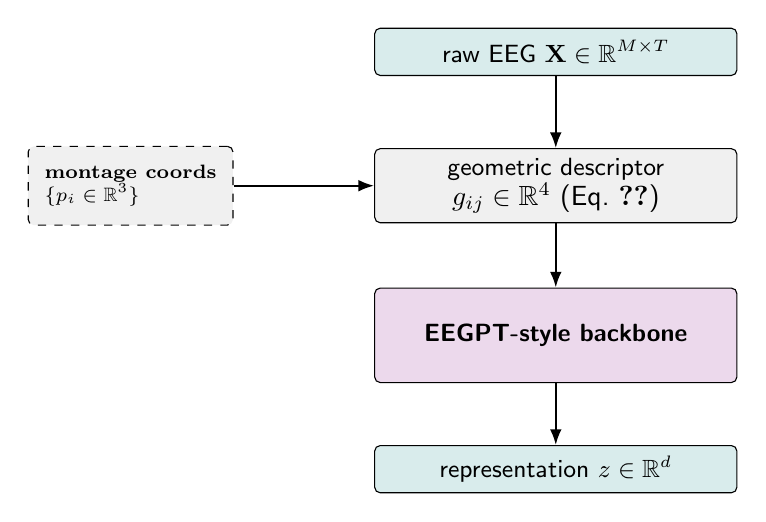
\begin{tikzpicture}[x=1cm, y=1cm]

    % --- Main vertical pipeline ---------------------------------------------
    \node[tealbox,  minimum width=4.6cm] (raw)   at (0,  0)
      {\small raw EEG  $\mathbf{X}\in\mathbb{R}^{M\times T}$};

    \node[graybox,  minimum width=4.6cm] (geo)   at (0, -1.7)
      {\small geometric descriptor\\[-1pt]
       $g_{ij} \in \mathbb{R}^4$ (Eq.~\ref{eq:geo_desc})};

    \node[purplebox,minimum width=4.6cm,minimum height=1.2cm] (eegpt) at (0, -3.6)
      {\small \textbf{EEGPT-style backbone}};

    \node[tealbox,  minimum width=4.6cm] (out)   at (0, -5.3)
      {\small representation  $z\in\mathbb{R}^d$};

    % --- Side input: coordinate table from montage --------------------------
    \node[graybox, minimum width=2.6cm, minimum height=1.0cm,
          align=left, font=\scriptsize, dashed] (coord) at (-5.4, -1.7)
      {\textbf{montage coords}\\
       $\{p_i \in \mathbb{R}^3\}$};

    % --- Forward arrows -----------------------------------------------------
    \draw[fwd] (raw)   -- (geo);
    \draw[fwd] (geo)   -- (eegpt);
    \draw[fwd] (eegpt) -- (out);
    \draw[fwd] (coord.east) -- (geo.west);

  \end{tikzpicture}
  \caption{\textbf{Architecture overview.} My contribution is the middle
  block: raw EEG plus the montage's electrode coordinates yield a geometric
  descriptor $g_{ij}$ that conditions the spatial attention of an otherwise
  standard EEGPT-style backbone. The codex of
  per-electrode embeddings used by EEGPT is removed; $g_{ij}$ takes its
  place as the spatial inductive bias. Coordinates are side information
  read from the recording montage --- digitized when available, otherwise
  taken from a 10--20 template.}
  \label{fig:arch}
\end{figure}
 inside a figure environment.
%            Assumes the same TikZ style header as review_fig_flow.tex
%            (tealbox, greenbox, bluebox, amberbox, purplebox, graybox,
%            fwd, ema, stopgrad).
%
%  DO NOT COMPILE. TikZ only.
%=============================================================================

\begin{figure}[h]
  \centering
  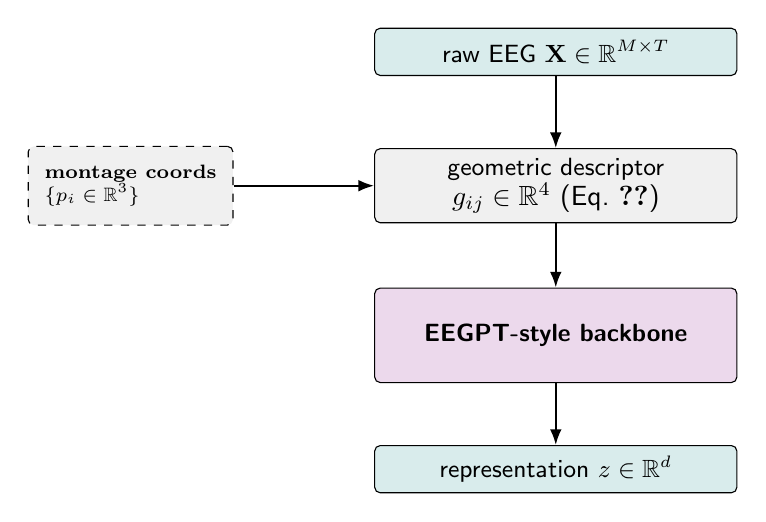
\begin{tikzpicture}[x=1cm, y=1cm]

    % --- Main vertical pipeline ---------------------------------------------
    \node[tealbox,  minimum width=4.6cm] (raw)   at (0,  0)
      {\small raw EEG  $\mathbf{X}\in\mathbb{R}^{M\times T}$};

    \node[graybox,  minimum width=4.6cm] (geo)   at (0, -1.7)
      {\small geometric descriptor\\[-1pt]
       $g_{ij} \in \mathbb{R}^4$ (Eq.~\ref{eq:geo_desc})};

    \node[purplebox,minimum width=4.6cm,minimum height=1.2cm] (eegpt) at (0, -3.6)
      {\small \textbf{EEGPT-style backbone}};

    \node[tealbox,  minimum width=4.6cm] (out)   at (0, -5.3)
      {\small representation  $z\in\mathbb{R}^d$};

    % --- Side input: coordinate table from montage --------------------------
    \node[graybox, minimum width=2.6cm, minimum height=1.0cm,
          align=left, font=\scriptsize, dashed] (coord) at (-5.4, -1.7)
      {\textbf{montage coords}\\
       $\{p_i \in \mathbb{R}^3\}$};

    % --- Forward arrows -----------------------------------------------------
    \draw[fwd] (raw)   -- (geo);
    \draw[fwd] (geo)   -- (eegpt);
    \draw[fwd] (eegpt) -- (out);
    \draw[fwd] (coord.east) -- (geo.west);

  \end{tikzpicture}
  \caption{\textbf{Architecture overview.} My contribution is the middle
  block: raw EEG plus the montage's electrode coordinates yield a geometric
  descriptor $g_{ij}$ that conditions the spatial attention of an otherwise
  standard EEGPT-style backbone. The codex of
  per-electrode embeddings used by EEGPT is removed; $g_{ij}$ takes its
  place as the spatial inductive bias. Coordinates are side information
  read from the recording montage --- digitized when available, otherwise
  taken from a 10--20 template.}
  \label{fig:arch}
\end{figure}
 inside a figure environment.
%            Assumes the same TikZ style header as review_fig_flow.tex
%            (tealbox, greenbox, bluebox, amberbox, purplebox, graybox,
%            fwd, ema, stopgrad).
%
%  DO NOT COMPILE. TikZ only.
%=============================================================================

\begin{figure}[h]
  \centering
  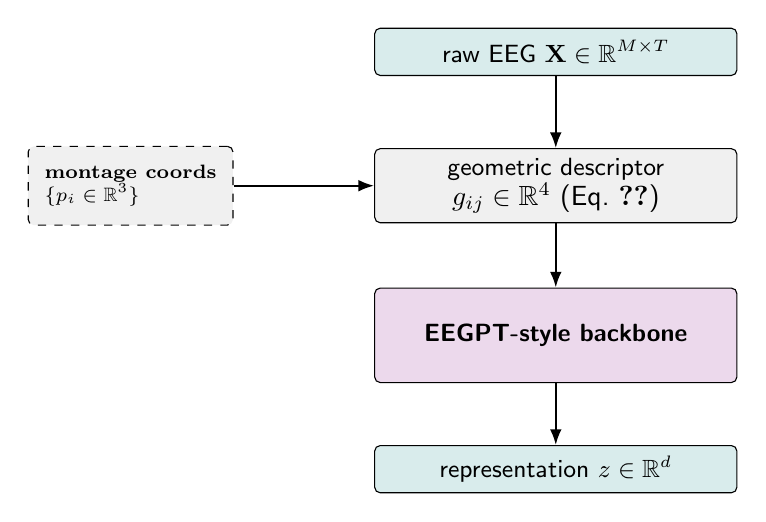
\begin{tikzpicture}[x=1cm, y=1cm]

    % --- Main vertical pipeline ---------------------------------------------
    \node[tealbox,  minimum width=4.6cm] (raw)   at (0,  0)
      {\small raw EEG  $\mathbf{X}\in\mathbb{R}^{M\times T}$};

    \node[graybox,  minimum width=4.6cm] (geo)   at (0, -1.7)
      {\small geometric descriptor\\[-1pt]
       $g_{ij} \in \mathbb{R}^4$ (Eq.~\ref{eq:geo_desc})};

    \node[purplebox,minimum width=4.6cm,minimum height=1.2cm] (eegpt) at (0, -3.6)
      {\small \textbf{EEGPT-style backbone}};

    \node[tealbox,  minimum width=4.6cm] (out)   at (0, -5.3)
      {\small representation  $z\in\mathbb{R}^d$};

    % --- Side input: coordinate table from montage --------------------------
    \node[graybox, minimum width=2.6cm, minimum height=1.0cm,
          align=left, font=\scriptsize, dashed] (coord) at (-5.4, -1.7)
      {\textbf{montage coords}\\
       $\{p_i \in \mathbb{R}^3\}$};

    % --- Forward arrows -----------------------------------------------------
    \draw[fwd] (raw)   -- (geo);
    \draw[fwd] (geo)   -- (eegpt);
    \draw[fwd] (eegpt) -- (out);
    \draw[fwd] (coord.east) -- (geo.west);

  \end{tikzpicture}
  \caption{\textbf{Architecture overview.} My contribution is the middle
  block: raw EEG plus the montage's electrode coordinates yield a geometric
  descriptor $g_{ij}$ that conditions the spatial attention of an otherwise
  standard EEGPT-style backbone. The codex of
  per-electrode embeddings used by EEGPT is removed; $g_{ij}$ takes its
  place as the spatial inductive bias. Coordinates are side information
  read from the recording montage --- digitized when available, otherwise
  taken from a 10--20 template.}
  \label{fig:arch}
\end{figure}


\subsection{The Geometric Descriptor}
\label{sec:solution:geometry}

For each ordered pair of electrodes $(i,j)$ with 3-D scalp coordinates
$p_i, p_j \in \mathbb{R}^3$, I define
\begin{equation}
  g_{ij} \;=\; \bigl[\,\|p_i - p_j\|_2,\; p_i - p_j\,\bigr]
        \;\in\; \mathbb{R}^4.
  \label{eq:geo_desc}
\end{equation}
The descriptor combines distance (a scalar that captures proximity) with
signed displacement (a 3-vector that distinguishes anterior from posterior
and left from right). It is asymmetric in $(i, j)$, so attention can express
directional preferences. Because $g_{ij}$ is a function of coordinates alone
and contains no electrode-identity parameters, the same descriptor space is
defined for any montage for which scalp coordinates are available.

\subsection{Geometric vs.\ Transductive Spatial Attention}
\label{sec:solution:contrast}

Figure~\ref{fig:inductive} contrasts the two designs. Writing the standard
dot-product attention as
$\alpha_{ij} \propto \exp\!\bigl((W_Q x_i)^{\!\top}(W_K x_j)/\sqrt{d}\bigr)$
with output $y_i = \sum_j \alpha_{ij} W_V x_j$, the three geometric variants
are:

%=============================================================================
%  fig_inductive.tex
%
%  FIGURE 2: Conceptual contrast between transductive (codex) attention and
%  geometric (inductive) attention.
%
%  Layout: two panels, left = codex, right = geometric.
%
%   LEFT  (codex / transductive)         RIGHT  (geometric / inductive)
%   --------------------------           -----------------------------
%   x_i  +  c_i  ->  token               x_i               -> token
%        ^                                                       |
%   electrode-indexed embedding          attention(token_i, token_j, g_ij)
%   added BEFORE attention               geometry enters the attention FUNCTION
%
%   attention is geometry-blind          no per-electrode parameters
%
%  USAGE:    %=============================================================================
%  fig_inductive.tex
%
%  FIGURE 2: Conceptual contrast between transductive (codex) attention and
%  geometric (inductive) attention.
%
%  Layout: two panels, left = codex, right = geometric.
%
%   LEFT  (codex / transductive)         RIGHT  (geometric / inductive)
%   --------------------------           -----------------------------
%   x_i  +  c_i  ->  token               x_i               -> token
%        ^                                                       |
%   electrode-indexed embedding          attention(token_i, token_j, g_ij)
%   added BEFORE attention               geometry enters the attention FUNCTION
%
%   attention is geometry-blind          no per-electrode parameters
%
%  USAGE:    %=============================================================================
%  fig_inductive.tex
%
%  FIGURE 2: Conceptual contrast between transductive (codex) attention and
%  geometric (inductive) attention.
%
%  Layout: two panels, left = codex, right = geometric.
%
%   LEFT  (codex / transductive)         RIGHT  (geometric / inductive)
%   --------------------------           -----------------------------
%   x_i  +  c_i  ->  token               x_i               -> token
%        ^                                                       |
%   electrode-indexed embedding          attention(token_i, token_j, g_ij)
%   added BEFORE attention               geometry enters the attention FUNCTION
%
%   attention is geometry-blind          no per-electrode parameters
%
%  USAGE:    \input{fig_inductive} inside a figure environment.
%            Assumes the same TikZ style header as review_fig_flow.tex.
%            Dashed boxes mark "electrode-specific" entry points.
%
%  DO NOT COMPILE. TikZ only.
%=============================================================================

\begin{figure}[h]
  \centering
  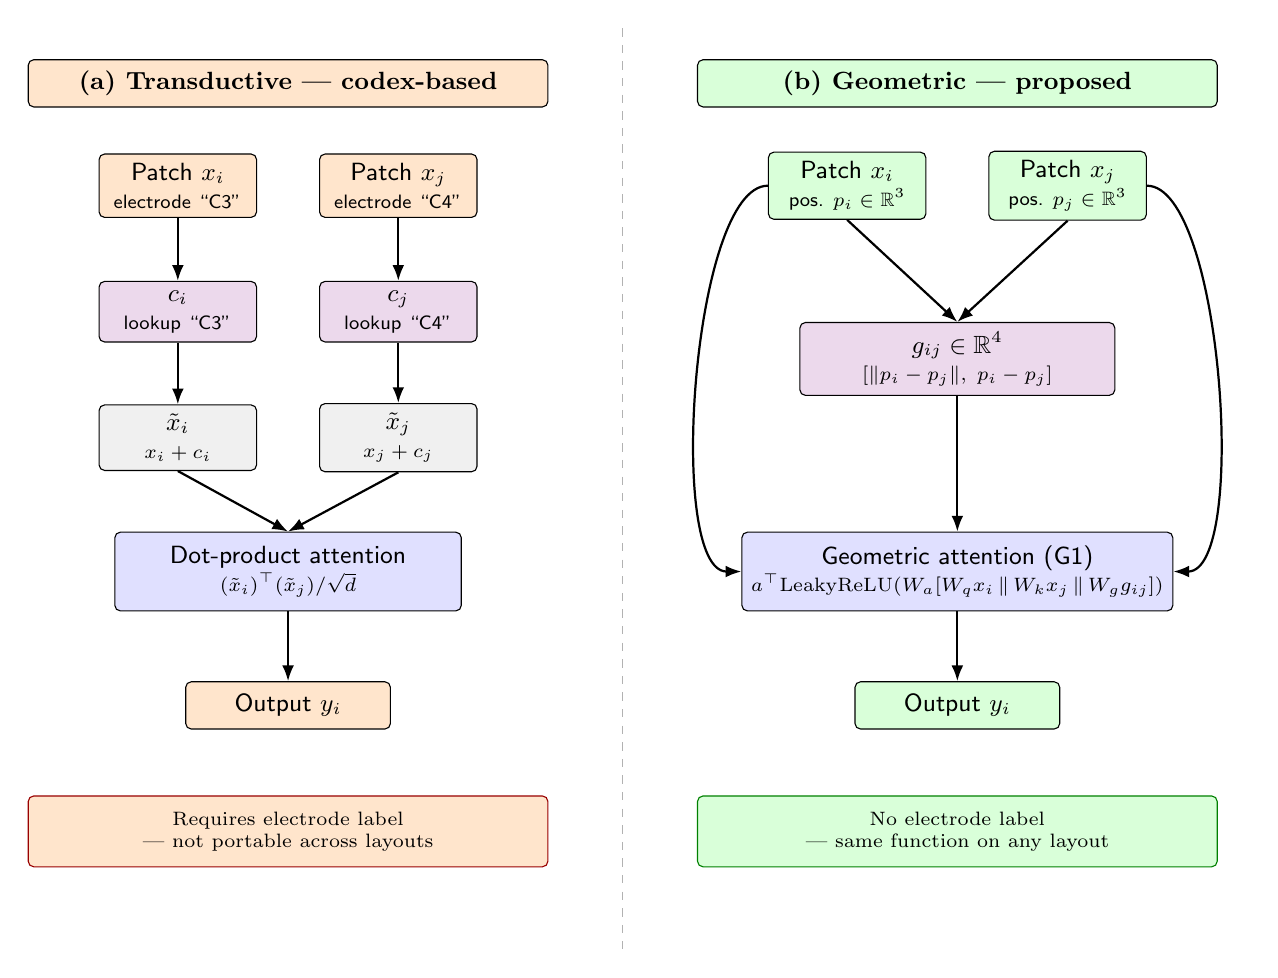
\begin{tikzpicture}[x=1cm, y=1cm]

    % ── Headers ───────────────────────────────────────────────────────────
    \node[amberbox, minimum width=6.6cm, font=\small\bfseries] (hdrL) at (0.0, 0.5)
      {(a) Transductive --- codex-based};
    \node[greenbox, minimum width=6.6cm, font=\small\bfseries] (hdrR) at (8.5, 0.5)
      {(b) Geometric --- proposed};

    % ── Dashed divider ───────────────────────────────────────────────────
    \draw[dashed, gray!60] (4.25, 1.2) -- (4.25, -10.5);

    % ════════════════════════════════════════════════════════════════════
    %  LEFT COLUMN: TRANSDUCTIVE
    % ════════════════════════════════════════════════════════════════════

    % Row 1: patch tokens with electrode LABELS as subtitle
    \node[amberbox, minimum width=2.0cm] (xiL) at (-1.4, -0.8)
      {\small Patch $x_i$\\[-2pt]\scriptsize electrode ``C3''};
    \node[amberbox, minimum width=2.0cm] (xjL) at ( 1.4, -0.8)
      {\small Patch $x_j$\\[-2pt]\scriptsize electrode ``C4''};

    % Row 2: codex lookups keyed by label
    \node[purplebox, minimum width=2.0cm] (ciL) at (-1.4, -2.4)
      {\small $c_i$\\[-2pt]\scriptsize lookup ``C3''};
    \node[purplebox, minimum width=2.0cm] (cjL) at ( 1.4, -2.4)
      {\small $c_j$\\[-2pt]\scriptsize lookup ``C4''};

    \draw[fwd] (xiL) -- (ciL);
    \draw[fwd] (xjL) -- (cjL);

    % Row 3: modified tokens (tilde x = x + c)
    \node[graybox, minimum width=2.0cm] (txiL) at (-1.4, -4.0)
      {\small $\tilde{x}_i$\\[-2pt]\scriptsize $x_i + c_i$};
    \node[graybox, minimum width=2.0cm] (txjL) at ( 1.4, -4.0)
      {\small $\tilde{x}_j$\\[-2pt]\scriptsize $x_j + c_j$};

    \draw[fwd] (ciL) -- (txiL);
    \draw[fwd] (cjL) -- (txjL);

    % Row 4: dot-product attention block
    \node[bluebox, minimum width=4.4cm, minimum height=1.0cm] (attL) at (0.0, -5.7)
      {\small Dot-product attention\\[-2pt]\scriptsize $(\tilde{x}_i)^\top (\tilde{x}_j)/\sqrt{d}$};

    \draw[fwd] (txiL.south) -- (attL.north);
    \draw[fwd] (txjL.south) -- (attL.north);

    % Row 5: output
    \node[amberbox, minimum width=2.6cm] (yL) at (0.0, -7.4)
      {\small Output $y_i$};
    \draw[fwd] (attL) -- (yL);

    % Bottom banner (red): label required
    \node[amberbox, minimum width=6.6cm, font=\scriptsize, align=center,
          minimum height=0.9cm, draw=red!60!black] (banL) at (0.0, -9.0)
      {Requires electrode label\\
       --- not portable across layouts};

    % ════════════════════════════════════════════════════════════════════
    %  RIGHT COLUMN: GEOMETRIC
    % ════════════════════════════════════════════════════════════════════

    % Row 1: patch tokens with COORDINATES as subtitle (no labels)
    \node[greenbox, minimum width=2.0cm] (xiR) at (7.1, -0.8)
      {\small Patch $x_i$\\[-2pt]\scriptsize pos. $p_i \in \mathbb{R}^3$};
    \node[greenbox, minimum width=2.0cm] (xjR) at (9.9, -0.8)
      {\small Patch $x_j$\\[-2pt]\scriptsize pos. $p_j \in \mathbb{R}^3$};

    % Row 2: g_ij computed directly from coordinates (no label step)
    \node[purplebox, minimum width=4.0cm] (gR) at (8.5, -3)
      {\small $g_{ij} \in \mathbb{R}^4$\\[-2pt]
       \scriptsize $[\|p_i - p_j\|,\; p_i - p_j]$};

    \draw[fwd] (xiR.south) -- (gR.north);
    \draw[fwd] (xjR.south) -- (gR.north);

    % Row 3: geometric attention block
    \node[bluebox, minimum width=5.4cm, minimum height=1.0cm] (attR) at (8.5, -5.7)
      {\small Geometric attention (G1)\\[-2pt]
       \scriptsize $a^\top \mathrm{LeakyReLU}(W_a [W_q x_i \,\|\, W_k x_j \,\|\, W_g g_{ij}])$};

    % Three inputs into the attention: x_i, x_j, g_ij
    \draw[fwd] (xiR.west) to[out=180, in=180, looseness=0.5] (attR.west);
    \draw[fwd] (xjR.east) to[out=0, in=0, looseness=0.5]  (attR.east);
    \draw[fwd] (gR)        --                  (attR);

    % Row 5: output
    \node[greenbox, minimum width=2.6cm] (yR) at (8.5, -7.4)
      {\small Output $y_i$};
    \draw[fwd] (attR) -- (yR);

    % Bottom banner (green): no label required
    \node[greenbox, minimum width=6.6cm, font=\scriptsize, align=center,
          minimum height=0.9cm, draw=green!50!black] (banR) at (8.5, -9.0)
      {No electrode label\\
       --- same function on any layout};

  \end{tikzpicture}
  \caption{\textbf{Transductive vs.\ inductive spatial attention.}
  Both panels start from the same EEG patches $x_i, x_j$ and arrive at an
  output $y_i$, but they route electrode information through different
  side channels. (a) The transductive baseline keys a learned codex by
  the electrode \emph{label} (``C3'', ``C4''), retrieving identity
  embeddings $c_i, c_j$ that are added to the patches before a standard
  dot-product attention. The codex table has one row per electrode seen
  during pretraining, so an unseen electrode has no entry. (b) The
  geometric encoder reads electrode \emph{positions} directly from the
  montage, computes the descriptor $g_{ij}$ from them, and feeds it into
  a shared attention function alongside the unmodified patches --- with
  no per-electrode parameters and no label dependency. The same function
  applies to any electrode pair given only its 3-D coordinates,
  including pairs from layouts never seen during pretraining.}
  \label{fig:inductive}
\end{figure}
 inside a figure environment.
%            Assumes the same TikZ style header as review_fig_flow.tex.
%            Dashed boxes mark "electrode-specific" entry points.
%
%  DO NOT COMPILE. TikZ only.
%=============================================================================

\begin{figure}[h]
  \centering
  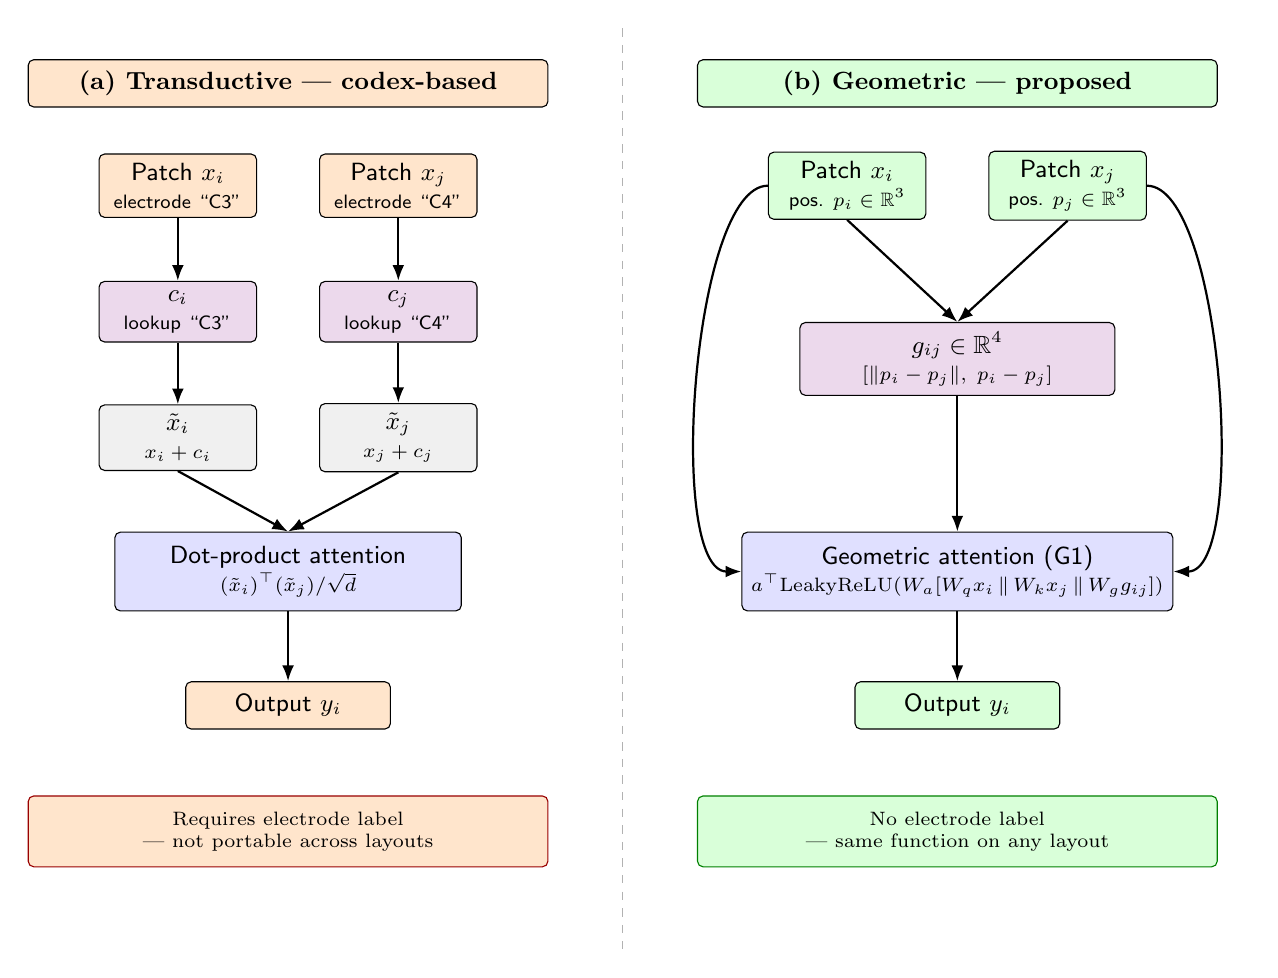
\begin{tikzpicture}[x=1cm, y=1cm]

    % ── Headers ───────────────────────────────────────────────────────────
    \node[amberbox, minimum width=6.6cm, font=\small\bfseries] (hdrL) at (0.0, 0.5)
      {(a) Transductive --- codex-based};
    \node[greenbox, minimum width=6.6cm, font=\small\bfseries] (hdrR) at (8.5, 0.5)
      {(b) Geometric --- proposed};

    % ── Dashed divider ───────────────────────────────────────────────────
    \draw[dashed, gray!60] (4.25, 1.2) -- (4.25, -10.5);

    % ════════════════════════════════════════════════════════════════════
    %  LEFT COLUMN: TRANSDUCTIVE
    % ════════════════════════════════════════════════════════════════════

    % Row 1: patch tokens with electrode LABELS as subtitle
    \node[amberbox, minimum width=2.0cm] (xiL) at (-1.4, -0.8)
      {\small Patch $x_i$\\[-2pt]\scriptsize electrode ``C3''};
    \node[amberbox, minimum width=2.0cm] (xjL) at ( 1.4, -0.8)
      {\small Patch $x_j$\\[-2pt]\scriptsize electrode ``C4''};

    % Row 2: codex lookups keyed by label
    \node[purplebox, minimum width=2.0cm] (ciL) at (-1.4, -2.4)
      {\small $c_i$\\[-2pt]\scriptsize lookup ``C3''};
    \node[purplebox, minimum width=2.0cm] (cjL) at ( 1.4, -2.4)
      {\small $c_j$\\[-2pt]\scriptsize lookup ``C4''};

    \draw[fwd] (xiL) -- (ciL);
    \draw[fwd] (xjL) -- (cjL);

    % Row 3: modified tokens (tilde x = x + c)
    \node[graybox, minimum width=2.0cm] (txiL) at (-1.4, -4.0)
      {\small $\tilde{x}_i$\\[-2pt]\scriptsize $x_i + c_i$};
    \node[graybox, minimum width=2.0cm] (txjL) at ( 1.4, -4.0)
      {\small $\tilde{x}_j$\\[-2pt]\scriptsize $x_j + c_j$};

    \draw[fwd] (ciL) -- (txiL);
    \draw[fwd] (cjL) -- (txjL);

    % Row 4: dot-product attention block
    \node[bluebox, minimum width=4.4cm, minimum height=1.0cm] (attL) at (0.0, -5.7)
      {\small Dot-product attention\\[-2pt]\scriptsize $(\tilde{x}_i)^\top (\tilde{x}_j)/\sqrt{d}$};

    \draw[fwd] (txiL.south) -- (attL.north);
    \draw[fwd] (txjL.south) -- (attL.north);

    % Row 5: output
    \node[amberbox, minimum width=2.6cm] (yL) at (0.0, -7.4)
      {\small Output $y_i$};
    \draw[fwd] (attL) -- (yL);

    % Bottom banner (red): label required
    \node[amberbox, minimum width=6.6cm, font=\scriptsize, align=center,
          minimum height=0.9cm, draw=red!60!black] (banL) at (0.0, -9.0)
      {Requires electrode label\\
       --- not portable across layouts};

    % ════════════════════════════════════════════════════════════════════
    %  RIGHT COLUMN: GEOMETRIC
    % ════════════════════════════════════════════════════════════════════

    % Row 1: patch tokens with COORDINATES as subtitle (no labels)
    \node[greenbox, minimum width=2.0cm] (xiR) at (7.1, -0.8)
      {\small Patch $x_i$\\[-2pt]\scriptsize pos. $p_i \in \mathbb{R}^3$};
    \node[greenbox, minimum width=2.0cm] (xjR) at (9.9, -0.8)
      {\small Patch $x_j$\\[-2pt]\scriptsize pos. $p_j \in \mathbb{R}^3$};

    % Row 2: g_ij computed directly from coordinates (no label step)
    \node[purplebox, minimum width=4.0cm] (gR) at (8.5, -3)
      {\small $g_{ij} \in \mathbb{R}^4$\\[-2pt]
       \scriptsize $[\|p_i - p_j\|,\; p_i - p_j]$};

    \draw[fwd] (xiR.south) -- (gR.north);
    \draw[fwd] (xjR.south) -- (gR.north);

    % Row 3: geometric attention block
    \node[bluebox, minimum width=5.4cm, minimum height=1.0cm] (attR) at (8.5, -5.7)
      {\small Geometric attention (G1)\\[-2pt]
       \scriptsize $a^\top \mathrm{LeakyReLU}(W_a [W_q x_i \,\|\, W_k x_j \,\|\, W_g g_{ij}])$};

    % Three inputs into the attention: x_i, x_j, g_ij
    \draw[fwd] (xiR.west) to[out=180, in=180, looseness=0.5] (attR.west);
    \draw[fwd] (xjR.east) to[out=0, in=0, looseness=0.5]  (attR.east);
    \draw[fwd] (gR)        --                  (attR);

    % Row 5: output
    \node[greenbox, minimum width=2.6cm] (yR) at (8.5, -7.4)
      {\small Output $y_i$};
    \draw[fwd] (attR) -- (yR);

    % Bottom banner (green): no label required
    \node[greenbox, minimum width=6.6cm, font=\scriptsize, align=center,
          minimum height=0.9cm, draw=green!50!black] (banR) at (8.5, -9.0)
      {No electrode label\\
       --- same function on any layout};

  \end{tikzpicture}
  \caption{\textbf{Transductive vs.\ inductive spatial attention.}
  Both panels start from the same EEG patches $x_i, x_j$ and arrive at an
  output $y_i$, but they route electrode information through different
  side channels. (a) The transductive baseline keys a learned codex by
  the electrode \emph{label} (``C3'', ``C4''), retrieving identity
  embeddings $c_i, c_j$ that are added to the patches before a standard
  dot-product attention. The codex table has one row per electrode seen
  during pretraining, so an unseen electrode has no entry. (b) The
  geometric encoder reads electrode \emph{positions} directly from the
  montage, computes the descriptor $g_{ij}$ from them, and feeds it into
  a shared attention function alongside the unmodified patches --- with
  no per-electrode parameters and no label dependency. The same function
  applies to any electrode pair given only its 3-D coordinates,
  including pairs from layouts never seen during pretraining.}
  \label{fig:inductive}
\end{figure}
 inside a figure environment.
%            Assumes the same TikZ style header as review_fig_flow.tex.
%            Dashed boxes mark "electrode-specific" entry points.
%
%  DO NOT COMPILE. TikZ only.
%=============================================================================

\begin{figure}[h]
  \centering
  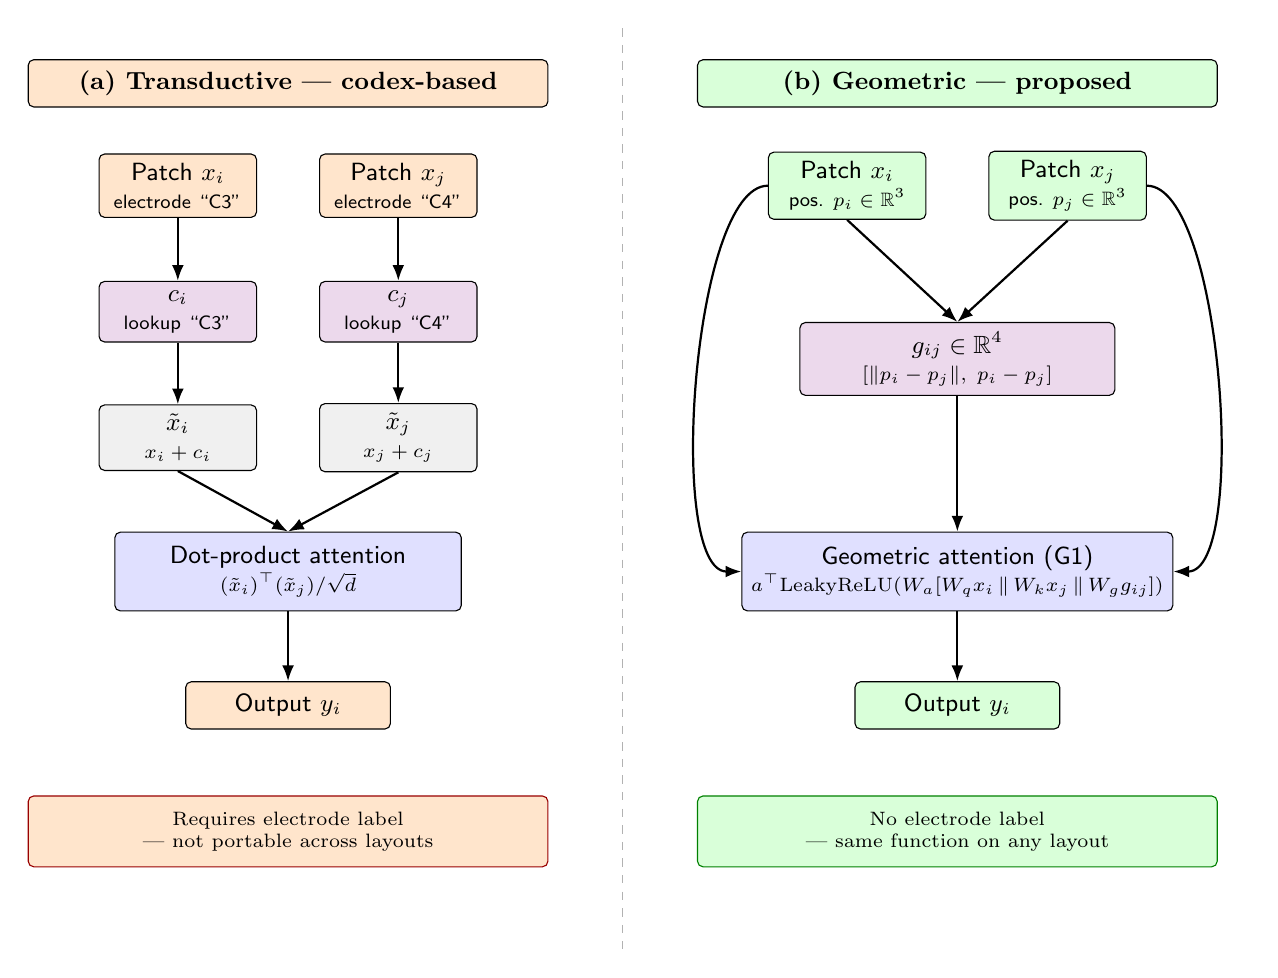
\begin{tikzpicture}[x=1cm, y=1cm]

    % ── Headers ───────────────────────────────────────────────────────────
    \node[amberbox, minimum width=6.6cm, font=\small\bfseries] (hdrL) at (0.0, 0.5)
      {(a) Transductive --- codex-based};
    \node[greenbox, minimum width=6.6cm, font=\small\bfseries] (hdrR) at (8.5, 0.5)
      {(b) Geometric --- proposed};

    % ── Dashed divider ───────────────────────────────────────────────────
    \draw[dashed, gray!60] (4.25, 1.2) -- (4.25, -10.5);

    % ════════════════════════════════════════════════════════════════════
    %  LEFT COLUMN: TRANSDUCTIVE
    % ════════════════════════════════════════════════════════════════════

    % Row 1: patch tokens with electrode LABELS as subtitle
    \node[amberbox, minimum width=2.0cm] (xiL) at (-1.4, -0.8)
      {\small Patch $x_i$\\[-2pt]\scriptsize electrode ``C3''};
    \node[amberbox, minimum width=2.0cm] (xjL) at ( 1.4, -0.8)
      {\small Patch $x_j$\\[-2pt]\scriptsize electrode ``C4''};

    % Row 2: codex lookups keyed by label
    \node[purplebox, minimum width=2.0cm] (ciL) at (-1.4, -2.4)
      {\small $c_i$\\[-2pt]\scriptsize lookup ``C3''};
    \node[purplebox, minimum width=2.0cm] (cjL) at ( 1.4, -2.4)
      {\small $c_j$\\[-2pt]\scriptsize lookup ``C4''};

    \draw[fwd] (xiL) -- (ciL);
    \draw[fwd] (xjL) -- (cjL);

    % Row 3: modified tokens (tilde x = x + c)
    \node[graybox, minimum width=2.0cm] (txiL) at (-1.4, -4.0)
      {\small $\tilde{x}_i$\\[-2pt]\scriptsize $x_i + c_i$};
    \node[graybox, minimum width=2.0cm] (txjL) at ( 1.4, -4.0)
      {\small $\tilde{x}_j$\\[-2pt]\scriptsize $x_j + c_j$};

    \draw[fwd] (ciL) -- (txiL);
    \draw[fwd] (cjL) -- (txjL);

    % Row 4: dot-product attention block
    \node[bluebox, minimum width=4.4cm, minimum height=1.0cm] (attL) at (0.0, -5.7)
      {\small Dot-product attention\\[-2pt]\scriptsize $(\tilde{x}_i)^\top (\tilde{x}_j)/\sqrt{d}$};

    \draw[fwd] (txiL.south) -- (attL.north);
    \draw[fwd] (txjL.south) -- (attL.north);

    % Row 5: output
    \node[amberbox, minimum width=2.6cm] (yL) at (0.0, -7.4)
      {\small Output $y_i$};
    \draw[fwd] (attL) -- (yL);

    % Bottom banner (red): label required
    \node[amberbox, minimum width=6.6cm, font=\scriptsize, align=center,
          minimum height=0.9cm, draw=red!60!black] (banL) at (0.0, -9.0)
      {Requires electrode label\\
       --- not portable across layouts};

    % ════════════════════════════════════════════════════════════════════
    %  RIGHT COLUMN: GEOMETRIC
    % ════════════════════════════════════════════════════════════════════

    % Row 1: patch tokens with COORDINATES as subtitle (no labels)
    \node[greenbox, minimum width=2.0cm] (xiR) at (7.1, -0.8)
      {\small Patch $x_i$\\[-2pt]\scriptsize pos. $p_i \in \mathbb{R}^3$};
    \node[greenbox, minimum width=2.0cm] (xjR) at (9.9, -0.8)
      {\small Patch $x_j$\\[-2pt]\scriptsize pos. $p_j \in \mathbb{R}^3$};

    % Row 2: g_ij computed directly from coordinates (no label step)
    \node[purplebox, minimum width=4.0cm] (gR) at (8.5, -3)
      {\small $g_{ij} \in \mathbb{R}^4$\\[-2pt]
       \scriptsize $[\|p_i - p_j\|,\; p_i - p_j]$};

    \draw[fwd] (xiR.south) -- (gR.north);
    \draw[fwd] (xjR.south) -- (gR.north);

    % Row 3: geometric attention block
    \node[bluebox, minimum width=5.4cm, minimum height=1.0cm] (attR) at (8.5, -5.7)
      {\small Geometric attention (G1)\\[-2pt]
       \scriptsize $a^\top \mathrm{LeakyReLU}(W_a [W_q x_i \,\|\, W_k x_j \,\|\, W_g g_{ij}])$};

    % Three inputs into the attention: x_i, x_j, g_ij
    \draw[fwd] (xiR.west) to[out=180, in=180, looseness=0.5] (attR.west);
    \draw[fwd] (xjR.east) to[out=0, in=0, looseness=0.5]  (attR.east);
    \draw[fwd] (gR)        --                  (attR);

    % Row 5: output
    \node[greenbox, minimum width=2.6cm] (yR) at (8.5, -7.4)
      {\small Output $y_i$};
    \draw[fwd] (attR) -- (yR);

    % Bottom banner (green): no label required
    \node[greenbox, minimum width=6.6cm, font=\scriptsize, align=center,
          minimum height=0.9cm, draw=green!50!black] (banR) at (8.5, -9.0)
      {No electrode label\\
       --- same function on any layout};

  \end{tikzpicture}
  \caption{\textbf{Transductive vs.\ inductive spatial attention.}
  Both panels start from the same EEG patches $x_i, x_j$ and arrive at an
  output $y_i$, but they route electrode information through different
  side channels. (a) The transductive baseline keys a learned codex by
  the electrode \emph{label} (``C3'', ``C4''), retrieving identity
  embeddings $c_i, c_j$ that are added to the patches before a standard
  dot-product attention. The codex table has one row per electrode seen
  during pretraining, so an unseen electrode has no entry. (b) The
  geometric encoder reads electrode \emph{positions} directly from the
  montage, computes the descriptor $g_{ij}$ from them, and feeds it into
  a shared attention function alongside the unmodified patches --- with
  no per-electrode parameters and no label dependency. The same function
  applies to any electrode pair given only its 3-D coordinates,
  including pairs from layouts never seen during pretraining.}
  \label{fig:inductive}
\end{figure}


\paragraph{G1 (score only).}
Geometry decides \emph{which} electrodes attend. The proposal wrote this in
GAT-style additive form
$e_{ij} = a^{\!\top}\mathrm{LeakyReLU}\!\bigl(W_a[W_Q x_i \,\|\, W_K x_j \,\|\, W_g g_{ij}]\bigr)$.
In my implementation G1 is realized as scaled dot-product attention with an
additive per-head geometric bias,
\begin{equation}
  e_{ij} = (W_Q x_i)^{\!\top}(W_K x_j)/\sqrt{d_h} + b_h(g_{ij}),
  \label{eq:opt1}
\end{equation}
where $b_h$ is a shared MLP $\mathbb{R}^4 \to \mathbb{R}^H$ (one output per
head). The motivation for this small deviation is to keep the geometric and
codex variants on the same attention kernel: the headline E1 comparison
then isolates the inductive-vs-transductive variable rather than confounding
it with additive-vs-dot-product attention. The literal GAT-additive form is
recoverable as a future ablation by swapping the kernel. G1 is the default
geometric variant on grounds of parsimony.

\paragraph{G2 (value only).}
Standard dot-product score; geometry-augmented value:
\begin{equation}
  v_{j \to i} = W_V x_j + W_{V,g}\, g_{ij},
  \qquad y_i = \sum_j \alpha_{ij}\, v_{j \to i}.
  \label{eq:opt2}
\end{equation}
Geometry colours \emph{what} messages carry, not who talks.

\paragraph{G3 (both).}
G1 score-side bias and G2 value-side addition, with separate projections
$W_g$ and $W_{V,g}$. Geometry simultaneously shapes which electrodes attend
and what they exchange. G3 is the most expressive variant and incurs the
largest geometric-parameter cost.

\subsection{Self-Supervised Objective}
\label{sec:solution:loss}

The encoder is supervised by the combination of momentum-encoder alignment
and optional masked-patch reconstruction:
\begin{equation}
  \mathcal{L} = \mathcal{L}_A + \lambda_R\, \mathcal{L}_R.
  \label{eq:loss}
\end{equation}
$\mathcal{L}_A$ is the alignment term,
$-2 \cdot \cos(\mathrm{pred}(z_\text{online}),\,\mathrm{stop\_grad}(z_\text{momentum}))$
averaged over batch and time. $\mathcal{L}_R$ is masked-patch reconstruction
MSE, applied only at masked time steps; the reconstruction target is the
channel-mean of the original patches. I default to $\lambda_R = 1$ with
50\% joint (electrode, time) masking. The momentum encoder is a
non-trainable EMA copy of the online encoder, processing the unmasked input.
The EMA factor follows a cosine ramp
$\tau(k) = 1 - (1 - \tau_0)\frac{\cos(\pi k / K) + 1}{2}$ with
$\tau_0 = 0.996$ and $\tau_K = 1.0$, matching the EEGPT recipe.

\subsection{Transductive Baseline}
\label{sec:solution:baseline}

Architecturally identical to the geometric encoder except for the spatial
mechanism: a learned codex $\{c_i \in \mathbb{R}^d\}$ is added to patch
projections before standard dot-product attention. At transfer time (E2c),
missing-electrode codex entries are populated by one of two fallbacks:
(a) \textbf{random}, $c_i \sim \mathcal{N}(0, \sigma^2)$ with $\sigma$
matched to the pretraining codex's empirical std; or
(b) \textbf{nearest-neighbour (nn)}, copying the codex entry of the
spatially-nearest pretraining electrode in \texttt{standard\_1005}
coordinates. The nn fallback effectively re-uses the pretraining geometry
at inference and is the strongest codex transfer baseline I evaluate.

\subsection{Why This Design Should Help (the Predicted Advantage)}
\label{sec:solution:why}

EEG non-stationarity --- across sessions, subjects, and montages --- is
largely a story of electrode geometry shifting. A model whose spatial
attention is a function of geometry absorbs that shift smoothly; a model
whose spatial structure lives in identity-indexed parameters cannot. Whether
the predicted advantage appears empirically, and whether its size justifies
any in-distribution cost, is what experiments E1 and E2 answer. The result,
reported in Section~\ref{sec:results}, is more nuanced than the proposal
anticipated.

% =============================================================================
\section{List of Experiments}
\label{sec:experiments}

I run the five-experiment plan committed to in the proposal. Two proposal
items not included here are E3 (channel-dropout curves) and E6
(loss-component ablation): both were marked optional in the proposal and
were dropped to fit the compute budget once the headline experiments were
under way.

\begin{table}[h]
\centering
\caption{Experiment overview.}
\label{tab:experiments}
\small
\begin{tabular}{p{0.6cm} p{5.0cm} p{3.5cm} p{4.5cm}}
\toprule
\textbf{ID} & \textbf{Question} & \textbf{Datasets} & \textbf{Variants} \\
\midrule
E1  & In-distribution linear-probe parity                & PhysioNet MI                   & G1, codex, channel-independent           \\
E2a & Cross-session within-subject (night~1 $\to$ night~2)& Sleep-EDFx                    & G1, codex                                \\
E2b & Cross-subject LOSO variance; paired Wilcoxon       & PhysioNet MI (full 105 subj)   & G1 vs.\ codex                            \\
E2c & Zero-shot cross-montage transfer (64\,ch $\to$ 3\,ch) & PhysioNet MI $\to$ BCIC-2B    & G1, codex-random, codex-nn               \\
E5  & Where $g_{ij}$ enters --- G1 / G2 / G3              & PhysioNet MI + BCIC-2B         & G1, G2, G3                               \\
E7  & Channel-independent sanity check                   & PhysioNet MI + BCIC-2B         & channel-independent, G1, codex           \\
\bottomrule
\end{tabular}
\end{table}

Each experiment is orchestrated by a dedicated script
(\texttt{scripts/run\_e1.py}, \texttt{scripts/run\_e2.py \{a,b,c\}},
\texttt{scripts/run\_e5.py}, \texttt{scripts/run\_e7.py}) that resolves a
checkpoint per variant, runs \texttt{scripts/probe.py} in a fresh subprocess,
and aggregates the BAC / $\kappa$ / weighted-F1 per subject into a JSON file
and a printed summary table. Variants without a finished checkpoint are
skipped with \texttt{(no ckpt)} and the table continues, so partial result
coverage is normal during iteration.

% =============================================================================
\section{Experimental Setup and Datasets}
\label{sec:setup}

\subsection{Datasets}
\label{sec:setup:datasets}

I use three open EEG datasets accessible through
MNE-Python~\cite{gramfort2013mne} and MOABB~\cite{aristimunha2023moabb}.

\begin{table}[h]
\centering
\caption{Open EEG datasets used in this project.}
\label{tab:datasets}
\small
\begin{tabular}{llrrrl}
\toprule
\textbf{Dataset} & \textbf{Paradigm} & \textbf{Subj.} & \textbf{Ch.} & \textbf{Rate} & \textbf{Used for} \\
\midrule
PhysioNet MI~\cite{schalk2004physionet}
  & Motor imagery (4-class)  & 109 $\to$ 105 & 64  & 160\,Hz  & E1, E2b, E5, E7, pretrain \\
BCIC-2B~\cite{tangermann2012bcic}
  & Motor imagery (binary)   &   9 &  3  & 250\,Hz  & E2c target, E5, E7 \\
Sleep-EDFx~\cite{kemp2000sleepedf}
  & Sleep staging (5-class)  & $\sim$78 & 2 bipolar & 100\,Hz & E2a \\
\bottomrule
\end{tabular}
\end{table}

Four PhysioNet MI subjects (88, 92, 100, 104) are excluded due to known
annotation/recording inconsistencies, leaving 105 subjects.

\paragraph{Why BCIC-2A was dropped.}
Despite the similar name, BCIC-2A and BCIC-2B are different datasets:
2A is 22-channel 4-class motor imagery on 9 subjects, while 2B is
3-channel binary motor imagery on 9 subjects. BCIC-2B is essential to this
project because its 3-channel layout (C3, Cz, C4) is the cross-montage
transfer target in E2c against the 64-channel PhysioNet MI pretraining
source; 2A's 22-channel layout would not provide a comparable montage
mismatch. BCIC-2A, on the other hand, would be a \emph{third} 4-class
motor-imagery dataset on top of PhysioNet MI (105 subjects, 4-class MI) ---
same paradigm, same task, with a 12$\times$ smaller cohort. Running it
would produce another in-distribution-style LOSO number on a tiny sample
with no new perturbation axis: cross-montage is already covered by 2B,
cross-subject by PhysioNet MI LOSO, and cross-session by Sleep-EDFx.
Dropping 2A was a compute-budget call, but the theoretical loss is small ---
the three perturbation axes the proposal committed to are fully covered
without it.

\subsection{Preprocessing (Tier 1, Locked Across Datasets)}
\label{sec:setup:preproc}

Identical preprocessing is applied to all three datasets so that
cross-dataset comparisons isolate dataset characteristics, not preprocessing
decisions:
\begin{itemize}[leftmargin=*, itemsep=2pt, topsep=2pt]
  \item Bandpass 0.5--45\,Hz, zero-phase FIR.
  \item Resample to 200\,Hz (PhysioNet 160 $\to$ up, BCIC 250 $\to$ down,
        Sleep-EDFx 100 $\to$ up; all end identical).
  \item Epoch length 4\,s (16 patches at 250\,ms per epoch).
  \item Per-epoch linear detrend, per-epoch per-channel z-score.
  \item No baseline correction, no re-referencing, no ICA.
  \item Montage: \texttt{standard\_1005}. Coordinate normalization:
        centroid-subtract, unit-max-norm scale.
\end{itemize}

The proposal initially listed 256\,Hz resample and 0.5--75\,Hz bandpass. I
locked Tier 1 to 200\,Hz and 0.5--45\,Hz instead. Both deviations have
explicit theoretical motivation. The 200\,Hz sampling rate is more than
twice the highest passband edge (45\,Hz), satisfying Nyquist with margin;
halving the sampling rate halves backbone compute and patch length at no
information cost over the 0.5--45\,Hz band. The 0.5--45\,Hz bandpass
excludes mains line noise (50/60\,Hz) cleanly and keeps the band wide enough
for both motor-imagery rhythms ($\mu$ 8--12\,Hz, $\beta$ 13--30\,Hz) and
sleep-staging features ($\delta$ 0.5--4\,Hz, $\theta$ 4--8\,Hz, sleep
spindles 11--16\,Hz). The deviation is logged in the project session log
and is consistent with the EEGPT preprocessing choice.

\paragraph{Sleep-EDFx specifics.}
The dataset uses two bipolar derivations (\texttt{Fpz--Cz},
\texttt{Pz--Oz}) that are not in any standard montage; I place each bipolar
electrode at the midpoint of its reference pair in \texttt{standard\_1005}
coordinates. Sleep-EDFx uses 30-second sleep-stage windows; I slice each
30\,s window into seven non-overlapping 4\,s sub-epochs, each inheriting the
parent label, to keep the backbone unchanged.

\paragraph{Artifact policy (Tier 3, asymmetric).}
Pretraining mode clips to $\pm 20\sigma$ after z-score (catches catastrophic
artifacts, leaves typical EOG/EMG for the model to learn to ignore).
Evaluation mode applies additional amplitude rejection at 100\,$\mu$V peak
per epoch.

\subsection{Architecture Defaults}
\label{sec:setup:arch}

Token dimension $d = 256$; spatial depth $L_S = 2$; temporal depth
$L_T = 4$; 8 heads; MLP ratio 4. Patch length 50 samples (250\,ms at
200\,Hz), non-overlapping; 16 patches per 4\,s epoch. Geometric MLPs:
hidden width 32. Temporal positional embedding: learned.

The geometric and transductive backbones share an identical
1.58\,M-parameter temporal-Transformer / projection / patcher stack. Only
the spatial encoder differs:

\begin{table}[h]
\centering
\caption{Distinguishing parameter counts at $d{=}256$, $H{=}8$, $L_S{=}2$,
$M{=}64$.}
\label{tab:params}
\small
\begin{tabular}{lr}
\toprule
\textbf{Variant} & \textbf{Distinguishing params} \\
\midrule
Geometric G1         &  848 \\
Geometric G2         & 17,216 \\
Geometric G3         & 18,064 \\
Transductive codex (full-rank) & 16,384 \\
Channel-independent  & 0 \\
\bottomrule
\end{tabular}
\end{table}

G2/G3 and codex are within $\sim$5\% of each other; G1 is roughly
19$\times$ smaller. I keep the codex at full rank (one
$\mathbb{R}^{256}$ vector per electrode) rather than nerfing it for exact
parity, since the full-rank codex is the standard formulation in LaBraM
and EEGPT and a nerfed codex would invite a ``you crippled the baseline''
critique.

\subsection{Training}
\label{sec:setup:training}

AdamW (lr $1{\cdot}10^{-3}$, weight decay 0.05); linear warmup for 10 epochs
then cosine decay to 0 over 100 total epochs; EMA $\tau$ cosine ramp
$0.996 \to 1.0$ over all steps; gradient clipping max-norm 1.0; batch size
64 epochs/step; $\lambda_R = 1$ with 50\% joint (electrode, time) masking.
Geometry tables are recomputed each training step because the geometric MLPs
are trainable; reusing a precomputed table across steps fails with
``backward through graph a second time'' since the graph is freed at
\texttt{loss.backward()}. At inference there is no backward, so geometry
tables are precomputed once per montage.

\subsection{Compute}
\label{sec:setup:compute}

Pretraining runs on Google Colab (T4 / A100); linear-probe evaluation runs
locally on Apple M-series MPS. Two scales appear in this document:
\textbf{pilot} (10 PhysioNet MI subjects, 100 epochs, $\sim$35\,min on MPS)
and \textbf{full} (105 PhysioNet MI subjects, 100 epochs, on Colab). Every
checkpoint is paired with a \texttt{config.yaml} containing the resolved
configuration (Tier 1 preprocessing, Tier 2 ablation flags, Tier 3 artifact
policy, training hyperparameters), so loading a checkpoint never relies on
source-code defaults.

\subsection{Linear-Probe Protocol}
\label{sec:setup:probe}

For each downstream evaluation: load the pretrained online backbone, freeze
all parameters; extract a fixed feature by mean-pooling the
temporal-Transformer output over its 16 time steps to obtain a single
$\mathbb{R}^{256}$ vector per epoch; fit
\texttt{sklearn.StandardScaler} on the training split only (no leakage into
test); fit
\texttt{sklearn.LogisticRegression(C{=}1, solver=`lbfgs', multi\_class=`multinomial')}.
Strictly linear --- no MLP probe --- so the result reflects representation
quality rather than probe capacity. Splits per protocol: LOSO (E1, E2b, E5,
E7); within-subject train-night-1 / test-night-2 (E2a); cross-montage
pretrain-on-64-channel then transfer-frozen-to-3-channel (E2c). The codex
baseline in E2c uses random or nearest-neighbour fallback for missing
electrodes; the geometric baseline transfers directly.

\subsection{Significance Testing}
\label{sec:setup:stats}

For E2b I run a paired Wilcoxon signed-rank test on per-subject BAC
differences between geometric (G1) and codex variants on PhysioNet MI LOSO,
using \texttt{scipy.stats.wilcoxon} at $\alpha = 0.05$.

% =============================================================================
\section{Results}
\label{sec:results}

All BAC values below are LOSO or within-subject means $\pm$ standard
deviations across subjects.

\subsection{E1 --- In-Distribution Linear Probe (PhysioNet MI)}
\label{sec:results:e1}

\begin{table}[h]
\centering
\caption{E1 --- PhysioNet MI LOSO BAC, 105 subjects, full scale.}
\label{tab:e1}
\small
\begin{tabular}{lcr}
\toprule
\textbf{Variant} & \textbf{Scale} & \textbf{LOSO BAC} \\
\midrule
Channel-independent   & full & 0.333 $\pm$ 0.064 \\
Transductive codex    & full & 0.341 $\pm$ 0.070 \\
Geometric G1          & full & 0.342 $\pm$ 0.067 \\
\bottomrule
\end{tabular}
\end{table}

The geometric and codex models are statistically indistinguishable
in-distribution. Both consistently beat the channel-independent control,
confirming that explicit spatial structure helps. Geometric attention pays
no in-distribution cost relative to the codex baseline --- this is the
fairness anchor that the proposal asked E1 to establish.

\subsection{E2 --- Robustness Ladder}
\label{sec:results:e2}

\subsubsection{E2a --- Cross-Session Within-Subject (Sleep-EDFx, night~1 $\to$ night~2)}

\begin{table}[h]
\centering
\caption{E2a --- Sleep-EDFx within-subject (train on night~1, test on night~2).}
\label{tab:e2a}
\small
\begin{tabular}{lcr}
\toprule
\textbf{Variant} & \textbf{Scale} & \textbf{Within-subject BAC} \\
\midrule
Geometric G1       & full & 0.532 $\pm$ 0.077 \\
Transductive codex & full & 0.533 $\pm$ 0.077 \\
\bottomrule
\end{tabular}
\end{table}

Geometric attention provides no measurable advantage on cross-session
transfer. This is the smallest geometric perturbation in the ladder (same
montage, different night, same subject). The proposal anticipated only a
modest gap here because session drift mixes the geometric component
(placement) with a non-geometric component (physiological state) that this
architecture does not address. The flat result is consistent with that
hedge.

\subsubsection{E2b --- Cross-Subject LOSO (PhysioNet MI, paired Wilcoxon)}

\begin{table}[h]
\centering
\caption{E2b --- PhysioNet MI LOSO BAC, 105 subjects.}
\label{tab:e2b}
\small
\begin{tabular}{lcr}
\toprule
\textbf{Variant} & \textbf{Scale} & \textbf{LOSO BAC} \\
\midrule
Geometric G1       & full & 0.342 $\pm$ 0.067 \\
Transductive codex & full & 0.341 $\pm$ 0.070 \\
\bottomrule
\end{tabular}
\end{table}

Paired Wilcoxon signed-rank test on per-subject BAC differences:
$W = 2695.5$, $p = 0.911$ --- not significant at $\alpha = 0.05$. I cannot
reject the null hypothesis that geometric and codex models have the same
per-subject BAC distribution on PhysioNet MI LOSO. The proposal anticipated
a robustness advantage for geometric attention in cross-subject transfer;
that advantage is not detectable at this scale.

\subsubsection{E2c --- Cross-Montage Zero-Shot Transfer (PhysioNet MI 64\,ch $\to$ BCIC-2B 3\,ch)}

\begin{table}[h]
\centering
\caption{E2c --- BCIC-2B LOSO BAC after zero-shot transfer from 64-channel
PhysioNet MI pretraining, 9 subjects.}
\label{tab:e2c}
\small
\begin{tabular}{lcr}
\toprule
\textbf{Variant} & \textbf{Scale} & \textbf{BCIC-2B LOSO BAC} \\
\midrule
Geometric G1                & full & 0.509 $\pm$ 0.028 \\
Transductive codex (random) & full & 0.513 $\pm$ 0.024 \\
\textbf{Transductive codex (nn)} & full & \textbf{0.525 $\pm$ 0.022} \\
\bottomrule
\end{tabular}
\end{table}

This is the proposal's headline experiment, and the result inverts the
predicted ordering. The codex baseline with random fallback already matches
the geometric encoder; the codex baseline with nearest-neighbour fallback
exceeds it by $\sim$1.6 BAC points. The nn fallback is, in effect,
\emph{reading the geometry at transfer time} and using it to assign each
unseen electrode the closest pretraining codex entry. It does so without
any of the parameter or computational overhead of the geometric attention
bias. At this scale, the codex baseline with nn fallback recovers most of
the inductive advantage that motivated the geometric attention mechanism.

\subsection{E5 --- Where $g_{ij}$ Enters (G1 vs.\ G2 vs.\ G3)}
\label{sec:results:e5}

\begin{table}[h]
\centering
\caption{E5 --- LOSO BAC across G1, G2, G3 on both PhysioNet MI (105 subj)
and BCIC-2B (9 subj).}
\label{tab:e5}
\small
\begin{tabular}{lrr}
\toprule
\textbf{Variant} & \textbf{PhysioNet MI LOSO BAC} & \textbf{BCIC-2B LOSO BAC} \\
\midrule
G1 (score)            & 0.342 $\pm$ 0.067 & 0.509 $\pm$ 0.028 \\
G2 (value)            & 0.343 $\pm$ 0.069 & 0.509 $\pm$ 0.026 \\
\textbf{G3 (both)}    & \textbf{0.350 $\pm$ 0.068} & \textbf{0.532 $\pm$ 0.025} \\
\bottomrule
\end{tabular}
\end{table}

G3 is consistently the best geometric variant on both datasets, with a
larger lead on BCIC-2B (+2.3 BAC over G1) than on PhysioNet MI (+0.8 BAC
over G1). G1 and G2 are statistically indistinguishable; their parameter
counts differ by 20$\times$ but their downstream BAC does not. The proposal
predicted G1 might be competitive on parsimony grounds; the data say the
extra capacity at both score and value is mildly but consistently helpful.

\subsection{E7 --- Channel-Independent Sanity Check}
\label{sec:results:e7}

\begin{table}[h]
\centering
\caption{E7 --- LOSO BAC across channel-independent, G1, and codex on both
PhysioNet MI and BCIC-2B.}
\label{tab:e7}
\small
\begin{tabular}{lrr}
\toprule
\textbf{Variant}         & \textbf{PhysioNet MI BAC} & \textbf{BCIC-2B BAC} \\
\midrule
Channel-independent      & 0.333 $\pm$ 0.064 & 0.500 $\pm$ 0.027 \\
Geometric G1             & 0.342 $\pm$ 0.067 & 0.509 $\pm$ 0.028 \\
\textbf{Transductive codex} & 0.341 $\pm$ 0.070 & \textbf{0.522 $\pm$ 0.024} \\
\bottomrule
\end{tabular}
\end{table}

Spatial structure helps consistently: both geometric and codex models beat
the channel-independent control on both datasets. On BCIC-2B specifically
the codex baseline beats G1 by a slightly larger margin than on PhysioNet
MI, consistent with the E2c finding that a well-formed codex is a stronger
baseline than the headline experiment anticipated.

\subsection{Headline Summary}
\label{sec:results:summary}

The proposal's central prediction was \emph{geometric $>$ transductive on
cross-montage transfer, ties in-distribution}. The actual result is
\emph{geometric $\approx$ transductive in-distribution, and slightly worse
than codex-with-nn on cross-montage transfer}. The strongest within-family
finding is that G3 is the best geometric variant on both datasets.

% =============================================================================
\section{Discussion}
\label{sec:discussion}

\subsection{What the Results Say Honestly}
Geometric attention is a competitive but not dominant alternative to a
codex-based spatial encoder at the scale evaluated here. In-distribution
there is no measurable difference (E1, E2b Wilcoxon). On the cross-montage
transfer that the proposal framed as the headline test, a codex baseline
equipped with a spatial nearest-neighbour fallback slightly beats the
geometric encoder (E2c). The strongest finding from this project is
therefore an \emph{internal} one: of the three geometric variants,
\textbf{G3 (geometry at both score and value)} dominates G1 and G2 on both
PhysioNet MI and BCIC-2B.

\subsection{Why the Headline Didn't Separate}
Three plausible explanations, in decreasing order of how much I trust them:

\paragraph{1. The codex-nn fallback exploits the same geometric prior at
transfer time.}
Replacing missing electrodes with their spatially-nearest pretraining
electrodes uses 3-D coordinates to drive the substitution. This is, in
effect, a one-step geometric prior layered on top of a transductive
backbone. It is cheaper than learning a geometric attention bias, and at
the scale of pretraining I could afford, it is enough.

\paragraph{2. Pilot-scale pretraining is below the data threshold where
inductive biases pay off.}
The full PhysioNet MI corpus is 105 subjects, which is small by
foundation-model standards. Inductive biases tend to help most when the
data is large enough that the network would otherwise overfit
identity-indexed parameters but small enough that capacity needs to be
shared across structurally-similar inputs. PhysioNet MI may simply not be
the regime where this trade-off bites.

\paragraph{3. The 4-D $g_{ij}$ descriptor is intentionally minimal and may
be insufficient.}
Distance + signed displacement does not encode hemisphere, gyrus, skull
conductivity, or cortical anatomy. The current null result is consistent
with the descriptor being too crude rather than the inductive framing being
wrong.

\subsection{What G3 Winning Tells Us About the Design Space}
G2 alone (geometry at the value) and G1 alone (geometry at the score) are
statistically tied on both datasets, despite a 20$\times$ difference in
distinguishing parameter count. G3 --- which adds both signals through
separate projections of the same $g_{ij}$ --- beats both. This suggests the
geometric advantage is not concentrated at any single point in the
attention computation; the cleanest reading is that geometry contributes a
small but consistent signal at \emph{each} slot it is allowed to enter,
and combining slots adds up. This is the most actionable finding from the
project, and the cleanest follow-up is to push G3 with richer descriptors.

\subsection{Relation to the Proposal Hypothesis}
The proposal phrased its expectation as ``I expect the transductive baseline
to remain competitive in-distribution, while geometric conditioning should
help most in cross-montage transfer.'' The first half held; the second did
not. I take the inversion as an informative result rather than a failed
one: it identifies a real, practical recipe --- codex + nearest-neighbour
fallback --- that captures most of the predicted inductive advantage at
lower implementation cost, and it gives the geometric line of work a
sharper target (beat \emph{codex-nn}, not naive codex).

% =============================================================================
\section{Conclusion}
\label{sec:conclusion}

I implemented and evaluated a geometrically inductive self-supervised EEG
encoder: spatial attention conditioned on a 4-D geometric descriptor
$g_{ij}$ instead of a learned per-electrode codex. I ran the full
evaluation plan committed to in the proposal --- in-distribution linear
probe (E1), three-step robustness ladder (E2a/b/c), G1/G2/G3 ablation
(E5), and channel-independent sanity check (E7) --- on three open EEG
datasets (PhysioNet MI, BCIC-2B, Sleep-EDFx).

The results do not support the proposal's central prediction that
geometric attention should dominate a transductive codex on robustness.
They support a more careful conclusion: spatial structure helps (both
geometric and codex beat channel-independent); the geometric and codex
variants are essentially tied in-distribution and on cross-subject LOSO;
and a codex baseline with a nearest-neighbour fallback at transfer time
slightly beats the geometric encoder on cross-montage transfer. The
strongest finding is internal to the geometric family: G3, with geometry
injected at both score and value, consistently dominates G1 and G2.

Framed as a design study, the project answers its research question ---
\emph{does geometric conditioning provide a robustness advantage over the
codex approach, and is that advantage large enough to matter?} --- with a
measured no, at the scale evaluated, and points to specific follow-ups
(richer descriptors, larger pretraining, high-density montages where
codex-nn breaks down) that could change the answer.

% =============================================================================
\section{Limitations}
\label{sec:limitations}

\begin{enumerate}[leftmargin=*, itemsep=3pt, topsep=2pt]
  \item \textbf{Pretraining scale.}
        PhysioNet MI is small by foundation-model standards (105 subjects,
        $\sim$14 runs per subject). Most EEG foundation-model papers
        pretrain on $10^3$--$10^4$ hours of recording; I am at $10^1$.
        Inductive-bias effects often grow with scale; this project cannot
        rule out that the geometric advantage materializes at LaBraM /
        EEGPT scale.
  \item \textbf{Single seed for most variants.}
        Time and compute did not permit multi-seed averaging for every
        variant; per-subject variance is reported but per-seed variance is
        not. Differences below $\sim$1 BAC point should be read cautiously.
  \item \textbf{Sleep-EDFx conflates geometric and physiological
        non-stationarity.}
        Section~\ref{sec:intro} was explicit about this: E2a measures a
        mixture of placement drift and physiological-state drift, and only
        the former is addressed by the architecture. The flat E2a result is
        consistent with the architecture working perfectly on the placement
        portion and gaining nothing on the state portion.
  \item \textbf{Minimal geometric descriptor.}
        $g_{ij} \in \mathbb{R}^4$ captures distance and signed displacement
        only. Richer descriptors --- spherical coordinates on the scalp
        sphere, hemisphere indicators, geodesic distance on a cortical
        mesh --- are listed as future work and are not evaluated.
  \item \textbf{Cross-montage evaluated at only one transfer point.}
        E2c measures 64-channel pretrain $\to$ 3-channel evaluation. The
        proposal mentioned a degradation curve across multiple levels of
        montage mismatch; only the endpoint is reported here.
  \item \textbf{G1 implementation is dot-product-plus-bias, not literal
        GAT-additive.}
        As described in Section~\ref{sec:solution:contrast}, this was a
        deliberate choice to share the attention kernel between geometric
        and codex variants and isolate the inductive-vs-transductive
        variable. The literal GAT-additive form was not evaluated.
  \item \textbf{No BCIC-2A.}
        Dropped to fit compute budget. The theoretical loss is small (see
        Section~\ref{sec:setup:datasets}); the three perturbation axes the
        proposal cared about are covered without it.
\end{enumerate}

% =============================================================================
\section{Future Work}
\label{sec:future}

The shape of the results points to three concrete follow-ups:

\paragraph{1.\ Richer geometric descriptors with G3.}
G3 was identified as the strongest geometric configuration. The natural
next step is to push G3 with a richer $g_{ij}$ --- spherical coordinates of
$p_i, p_j$, an explicit hemisphere indicator, or geodesic distance computed
on a cortical-surface mesh. The current 4-D descriptor is intentionally the
smallest sensible choice; if geometry helps at all, a richer descriptor
with the strongest variant is where the next BAC points should come from.

\paragraph{2.\ Scale-up pretraining and re-run E2c.}
The most informative single experiment to settle the headline question is
to scale pretraining beyond pilot scale --- at minimum to LaBraM-style
multi-thousand-hour corpora --- and re-run E2c. If the geometric advantage
over codex-nn appears at scale, that would confirm the inductive-bias
story; if not, the codex-nn baseline is genuinely competitive and the
proposal's central claim is mis-targeted.

\paragraph{3.\ High-density montage transfer where codex-nn breaks down.}
Codex-nn substitutes the \emph{single} nearest pretraining electrode. At
$M \geq 128$ the local electrode density is high enough that ``the nearest
neighbour'' is almost the same as ``the electrode itself''; at very
different montages (clinical 19-channel layouts, sparse consumer headsets)
the nn substitution becomes a coarser approximation. The proposal flagged
$M \geq 128$ as the regime where kNN attention sparsification might begin
to matter; the same regime is also where codex-nn fallback should begin to
break down. Constructing this transfer carefully would isolate whether
geometric attention dominates in the limit where the nn shortcut fails.

\paragraph{Smaller follow-ups.}
(a) Implement the literal GAT-additive G1 and confirm it matches
dot-product-plus-bias G1; (b) implement the full E2c degradation curve
across multiple intermediate montages; (c) ablate $\lambda_R$ and the
masking strategy, which the proposal listed as E6 but was dropped for
compute reasons.

% =============================================================================
\section{Contributions}
\label{sec:contributions}

This is a \textbf{single-author project}. All design, implementation,
experiments, and writing are by Tianxin Zhou. No collaborators contributed
code or text.

I used GitHub Copilot and Claude Code as coding assistants during
implementation: pairing on smoke-test scaffolds, refactors, and
documentation. The architectural decisions, experimental design, dataset
choices, and the analysis of the results in this report are mine. Where the
assistant drafted prose, I rewrote it before inclusion. The course's policy
that ``using gen-AI solely to generate your project report \ldots\ will
result in you failing the course'' is the boundary I operated within: the
engineering work, the experimental judgement, and the honest framing of the
negative-leaning headline result are my own.

% =============================================================================
\section{Reused Open-Source Code}
\label{sec:reused}

\begin{itemize}[leftmargin=*, itemsep=2pt, topsep=2pt]
  \item \textbf{EEGPT}~\cite{wang2024eegpt} ---
        \href{https://github.com/BINE022/EEGPT}{github.com/BINE022/EEGPT}.
        I read the EEGPT codebase to validate (a) the cosine ramp for the
        EMA $\tau$ schedule, (b) stop-gradient placement in the alignment
        loss, and (c) the channel-mean target convention for masked-patch
        reconstruction. The EEGPT repository is licensed Apache 2.0 and is
        cloned at the project root for reference; my code is an independent
        implementation, not a fork.
  \item \textbf{MNE-Python}~\cite{gramfort2013mne} --- data loading,
        montage handling, EDF parsing, bandpass filtering, resampling.
  \item \textbf{MOABB}~\cite{aristimunha2023moabb} --- BCIC-2B dataset
        access (\texttt{BNCI2014\_004}).
  \item \textbf{PyTorch} --- backbone, attention, training loop.
  \item \textbf{scikit-learn} --- \texttt{StandardScaler},
        \texttt{LogisticRegression}, balanced accuracy / Cohen's $\kappa$
        scoring.
  \item \textbf{SciPy} --- \texttt{scipy.stats.wilcoxon} for the paired
        test in E2b.
\end{itemize}

The project itself is licensed under the LICENSE file in the public
repository at
\href{https://github.com/tianxin-scu/geometric-eeg-ssl}{github.com/tianxin-scu/geometric-eeg-ssl}.

% =============================================================================
\bibliographystyle{abbrv}
{\footnotesize
\bibliography{references}
}

\end{document}
